\documentclass[12pt]{extarticle}
\usepackage[framemethod=TikZ]{mdframed}
\usepackage{amsthm}
\usepackage{tcolorbox}
\usepackage[margin=0.75in]{geometry}
\usepackage{setspace}
\usepackage{amsmath}
\usepackage{cancel}
\usepackage{multicol}
\def\deg{\ensuremath{^\circ}}
\def\v#1{\ensuremath{\mathrm{#1}}}
\usepackage{multirow}
\usepackage{fancyhdr}
\pagestyle{fancy}
\usepackage{lastpage} 
\usepackage{colortbl}
\usepackage{amssymb}
\usepackage{graphicx}
\setlength{\parskip}{0pt}
\lhead{Jhon Christian N. Rozano}
\chead{}
\rhead{May 24, 2021}

\lfoot{Source: Brilliant}
\cfoot{}
\rfoot{Page \thepage\ of \pageref{LastPage}}

\renewcommand{\headrulewidth}{1pt}

\renewcommand{\footrulewidth}{1pt}

\newcommand*\Eval[3]{\left.#1\right\rvert_{#2}^{#3}}

\definecolor{LightCyan}{rgb}{0.88,1,1}

\renewcommand{\familydefault}{\sfdefault}


\begin{document}
	\setlength{\columnsep}{10pt}
	\renewcommand{\arraystretch}{1.5}
	\singlespacing
	\newtcolorbox{mybox}[1]{title=#1}
	
	\begin{center}
		{\large  \textbf{Physics Problems of the Day}} \\ 
	\end{center}
	\textbf{Problem 1:} On a school trip, Otto tries to take a selfie with the bottom of a deep well, but the phone slips out of his hand and into the well. He drops the phone \( 10\text{ m}  \) above the water's surface, and he listens for the splash from the same height. How many seconds will it take before Otto hears the splash? \\
	\textbf{Note:} Assume no air resistance, \( g = 9.81{\text{ m/s}}^2 \), and the speed of sound equal to \(343\text{ m/s}\).
	
	\begin{mybox}{\textbf{Solution}}
		Let $t$ be the time it takes to travel $10\text{ m}$ below the well. Then applying kinematics equation, we get
		\[ \Delta x = \frac{1}{2}at^2 \Rightarrow 10 = \frac{1}{2}\times 9.81\text{ m/s}^2 \times t^2  \]
		Therefore, \( t \approx 1.43\text{ s} \). After the phone drops into the well, the sound will also travel \(10\text{ m} \), reaching Otto's ears. Since the time is equal to distance divided by speed, we get
		\[ t_1 = \frac{\text{distance}}{\text{speed}} = \frac{10\text{ m}}{343\text{ m/s}} \approx 0.03\text{ s}\]
		Thus, the total time it will take before Otto hears the splash is 
		\[ t_\text{total} = 1.43\text{ s} + 0.03\text{ s} = \boxed{1.46\text{ s}} \]
	\end{mybox}

	\noindent \textbf{Problem 2:} 
	\begin{center}
		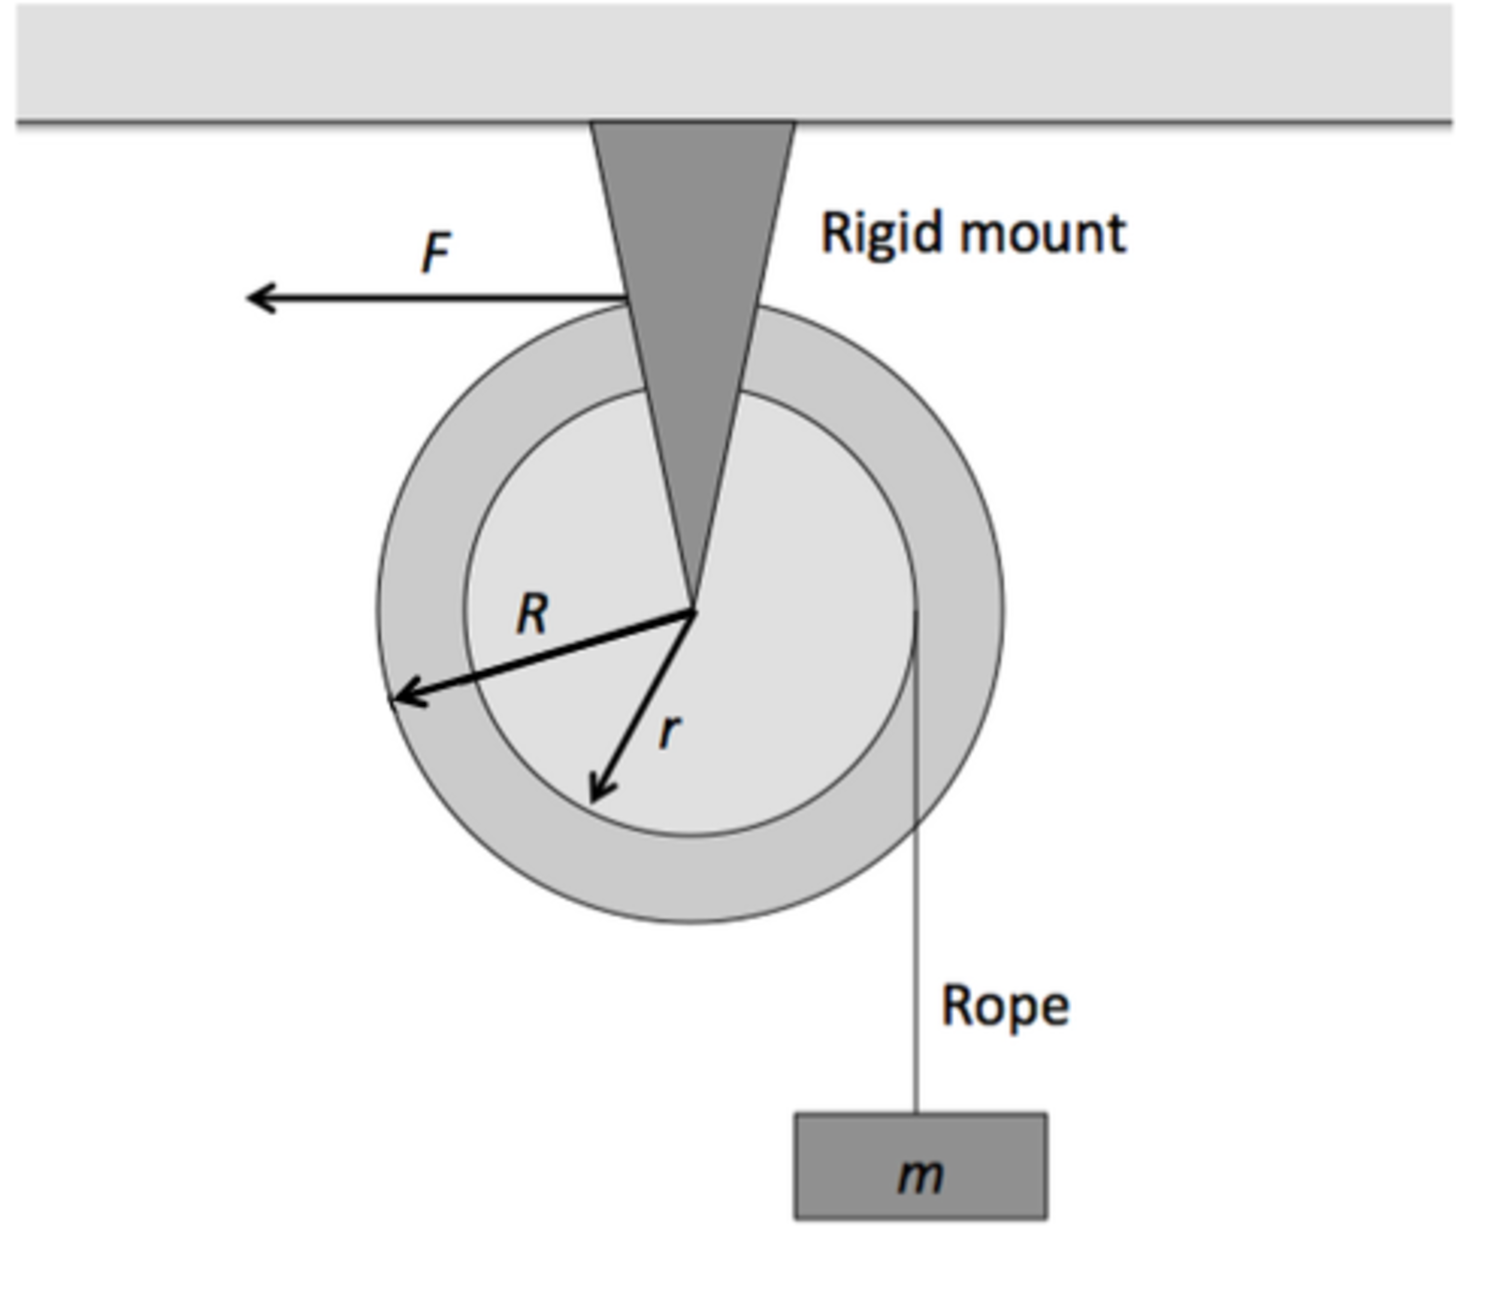
\includegraphics[clip=true, scale=0.09]{5b29986a80.6065de92f1.DdtrKM.png}
	\end{center}
	
	\begin{mybox}{\textbf{Solution}}
		Let $t$ be the time it takes to travel $10\text{ m}$ below the well. Then applying kinematics equation, we get
		\[ \Delta x = \frac{1}{2}at^2 \Rightarrow 10 = \frac{1}{2}\times 9.81\text{ m/s}^2 \times t^2  \]
		Therefore, \( t \approx 1.43\text{ s} \). After the phone drops into the well, the sound will also travel \(10\text{ m} \), reaching Otto's ears. Since the time is equal to distance divided by speed, we get
		\[ t_1 = \frac{\text{distance}}{\text{speed}} = \frac{10\text{ m}}{343\text{ m/s}} \approx 0.03\text{ s}\]
		Thus, the total time it will take before Otto hears the splash is 
		\[ t_\text{total} = 1.43\text{ s} + 0.03\text{ s} = \boxed{1.46\text{ s}} \]
	\end{mybox}
	
	
\end{document}
